\documentclass[11pt]{article}
\usepackage[margin=1in]{geometry}
\usepackage[none]{hyphenat}
\usepackage{fancyhdr}
\pagestyle{fancy}
\fancyhead{}
\fancyfoot{}
\fancyhead[C]
{\textbf{LOVISH MEHTA}}                          % Name

\usepackage{graphicx}
\usepackage{enumitem}

\begin{document}

\noindent\begin{minipage}{0.5\textwidth}      
\begin{flushleft}
H.No. 709, \\                                      % Address            
Sec-5,Urban Estate,\\
Kurukshetra-136118,\\
Haryana
\end{flushleft}
\end{minipage}
\noindent\begin{minipage}{0.5\textwidth}
\begin{flushright}                                 % Contact details     
     Contact  : 9517732414\\
e-mail id: mehtalovish76@gmail.com\\
\end{flushright}
\end{minipage}

\begin{flushright}
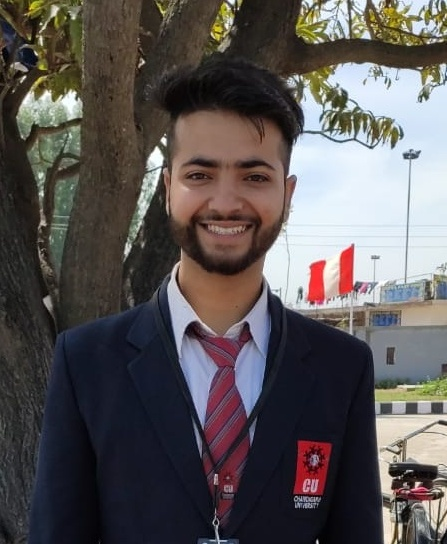
\includegraphics[scale=0.18]{profile.jpeg}      % Photograph
\end{flushright}


% Objective Section
\section{Objective}
To be a part of the organization that offers professional growth while being resourceful , innovative , and flexible.To have challenging career where I can fully explore my abilities and skills and to make significant contribution to the success of the employer and at the same time my own while working in a team\\

% Education Section
\section{Education}
\begin{flushright}

\begin{tabular}{||l|l|c|r|r||}
\hline
Degree & College/School  & Passing Year & Pass Percentage \\
\hline 
10th & Maharana Pratap Public School & 2014 & 91.6\\
12th & Maharana Pratap Public School & 2016 & 71.2\\
B.Tech & Chandigarh University & 2020 & 76.9\\
\hline
\end{tabular}
 \end{flushright} 

%Project Section
\section{Projects}
\begin{enumerate}[label=(\arabic*)]

\item\textbf{Individual Identification using Computer Vision and Augmented Reality}:\\
This project idea is to replace present College ID Cards with the new ID cards having aruco marker on them so that they can be identified easily with the help of camera.

\item\textbf{Eyantra Project(eYRC 2019)}:\\
 Responsibilities:\\
1.Interfacing of IR sensor ,motors, encoders and Xbee module with ATMEGA2560 microcontroller and writting code for line following in embedded C.\\
2.Designing Orientation Algorithm which helps the bot to decide which direction to face after reaching destination point.

\item\textbf{ Air Pollution Monitor} :\\
 This project includes making of a device which measures the count of various particulate matter  present in the surrounding air.\\
The section of the project I worked on are as follows :\\
i)  Interfacing Various sensors like BME-280,CCS811,PMS7003,Telaire T6700 with Atmega328p microcontroller.\\
ii) Using various communication protocols such as I2C, UART and SPI.\\
iii)Working on the graphics of TFT screen and interfacing it with the Atmega328p.

\item\textbf{PCB }(for Air Pollution Monitior) :\\
I designed two PCB's for the prototype of the Air Pollution Monitor. The PCB had connection for 1.8 TFT screen, Atmega328p micro-controller, PMS sensor, Charging circuit, Voltage booster circuit etc.

\item\textbf{Line Imitator} :\\
Line Imitator project included use of Arduino Atmega2560,IR sensors and DC motors together to follow the white line on black surface. For efficient line following I used a feedback algorithm which returned the relative position of IR sensors with respect to the white line and bot adjusted itself above the line according to the values.

\item\textbf{IARC} :\\
IARC bot performed three major functions:\\
1.Wall following : Following the wall with help of Ultrasonic Sensor.\\
2.Line following : Following the black line on white surface using IR Senors.\\
3.Color Recognition :  Differentiating b/w Blue and Red boxes using TCS3200 Sensor.\\                                     
All the sensor were interfaced with the Arduino Atmega2560.

\item\textbf{Remote Controlled Hydraulic Arm} :\\
In this project I modified the Hydraulic arm made with the help of Syringes by adding a remote controlled mechanism in it. The mechanism pushes and pulls the barrel of the syringe. Mechanism involves use of DC motors, long Screws and bolts. Also I used HC05 bluetooth module and Arduino Uno for the communication between Remote and Dc motors.

\item\textbf{Women Protection glove} :\\
I made a women protection Glove which was for the purpose of the women security.
It's a Shock glove which can be worn as a normal glove and can be used as a teaser for self defence.
\end{enumerate}

\section{Internships} 
\begin{itemize}
\item\textbf{Aerogram Pvt. Ltd.} IIT Delhi :\\
Dec 2018 - Jan 2019\\
During my internship I designed industrial level two PCB's for a product .Also I worked on micro-python board which is one of the new micro-controller boards in the market and made a prototype of a product as per company requirements.
 
\item\textbf{Phase Laboratories Pvt. Ltd.} IIT Delhi :\\
Jun 2018 - Jul 2018\\
During my internship I worked on a product for which i interfaced many sensor together like CCS-811,, BME-280, Telaire T6713 , TFT screen , PMS7003 etc using STM-32 microcontroller. I also merged all the codes of different sensors into one code.

\item\textbf{HBeonlabs Technologies Pvt. Ltd.},Greater Noida :\\ 
May 2018 - Jun 2018\\
I worked as an embbeded engineer in the respected company. There i worked on B.Tech projects using 8051 micro-controller.

\end{itemize}

\section{Research Publication}
\textbf{None}

\section{Technical Skills}
\begin{itemize}
\item\textbf{C Programming}
\item\textbf{C++ Programming}
\item\textbf{Python}
\item\textbf{Atmel avr}
\item\textbf{Arduino}
\item\textbf{PCB designing}
\item\textbf{KiCAD}
\item\textbf{Embedded Systems}
\end{itemize}

\section{Soft Skills}
\begin{itemize}
\item\textbf{Leadership}
\item\textbf{Confident}
\item\textbf{Problem solving}
\item\textbf{dedicated}
\item\textbf{Multitasking}
\item\textbf{Time management}
\item\textbf{Able to work in a busy and varied atmosphere }
\end{itemize}

\section{Co-ciricular Activities}
\textbf{1. Won first prize in Line Imitator Competition at IIT Ropar}\\\\
\textbf{2. a)Won first prize in inter department Abdul Kalam innovation Competition- 2017,Chandigarh University,Chandigarh }\\
\textbf{ b)Won first prize in inter department Abdul Kalam innovation Competition - 2018,Chandigarh University,Chandigarh }\\
\textbf{ c)Won third prize in inter department Abdul Kalam innovation, Competition- 2019,Chandigarh University,Chandigarh }\\\\
\textbf{3. Won Second prize for presenting Remote Controlled Hydraulic Arm on occassion of Engineers Day,Chandigarh University,Chandigarh }\\\\
\textbf{4. Participated in IARC Robotics competition hedl at IIT kanpur 2018, Kanpur} \\\\

\section{Extra-ciricular Activities}
\textbf{ Participated in 5 K.M. Marathon in 2017 held at Sukhna Lake, Chandigarh}}
\end{document}